%
% teil2.tex -- Beispiel-File für teil2 
%
% (c) 2020 Prof Dr Andreas Müller, Hochschule Rapperswil
%
\section{Klothoide
\label{fresnel:section:klothoide}}
\rhead{Klothoide}
In diesem Abschnitt soll gezeigt werden, dass die Krümmung der 
Euler-Spirale proportional zur vom Nullpunkt aus gemessenen Bogenlänge
ist.

\begin{definition}
Eine ebene Kurve, deren Krümmung proportionale zur Kurvenlänge ist,
heisst {\em Klothoide}.
\end{definition}

Die Klothoide wird zum Beispiel im Strassenbau für Autobahnkurven
verwendet.
Fährt man mit konstanter Geschwindigkeit entlang einer Klothoide,
muss man die Krümmung mit konstaner Geschwindigkeit ändern,
also das Lenkrad mit konstanter Geschwindigkeit drehen.
Dies ermöglicht eine ruhige Fahrweise.

\subsection{Krümmung einer ebenen Kurve}
\begin{figure}
\centering
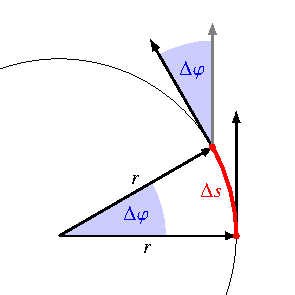
\includegraphics{papers/fresnel/images/kruemmung.pdf}
\caption{Berechnung der Krümmung einer ebenen Kurve.
\label{fresnel:figure:kruemmung}}
\end{figure}
Abbildung~\ref{fresnel:figure:kruemmung} erinnert daran, dass der
Bogen eines Kreises vom Radius $r$, entlang dem sich die Richtung
der Tangente um $\Delta\varphi$ ändert, die Länge
$\Delta s = r\Delta\varphi$.
Die Krümmung ist der Kehrwert des Krümmungsradius, daraus kann
man ablesen, dass 
\[
\kappa = \frac{1}{r} = \frac{\Delta \varphi}{\Delta s}.
\]
Für eine beliebige ebene Kurve ist daher die Krümmung
\[
\kappa = \frac{d\varphi}{ds}.
\]

\subsection{Krümmung der Euler-Spirale}
Wir betrachten jetzt die Euler-Spirale mit der Parametrisierung
$\gamma(s) = (C_1(s),S_1(s))$.
Zunächst stellen wir fest, dass die Länge der Tangente
\[
\dot{\gamma}(s)
=
\frac{d\gamma}{ds}
=
\begin{pmatrix}
\dot{C}_1(s)\\
\dot{S}_1(s)
\end{pmatrix}
=
\begin{pmatrix}
\cos s^2\\
\sin s^2
\end{pmatrix}
\qquad\Rightarrow\qquad
|\dot{\gamma}(s)|
=
\sqrt{\cos^2s^2+\sin^2s^2}
=
1.
\]
Insbesondere ist der Parameter $s$ der Kurve $\gamma(s)$ die
Bogenlänge.

Der zu $\dot{\gamma}(s)$ gehörige Polarwinkel kann aus dem Vergleich
mit einem Vektor mit bekanntem Polarwinkel $\varphi$ abgelesen werden:
\[
\begin{pmatrix}
\cos \varphi\\
\sin \varphi
\end{pmatrix}
=
\dot{\gamma}(s)
=
\begin{pmatrix}
\cos s^2\\\sin s^2
\end{pmatrix},
\]
der Polarwinkel 
ist daher $\varphi = s^2$.
Die Krümmung ist die Ableitung des Polarwinkels nach $s$, also
\[
\kappa
=
\frac{d\varphi}{ds}
=
\frac{ds^2}{ds}
=
2s,
\]
sie ist somit proportional zur Bogenlänge $s$.
Damit folgt, dass die Euler-Spirale eine Klothoide ist.

\subsection{Eine Kugel schälen}
\begin{figure}
\centering
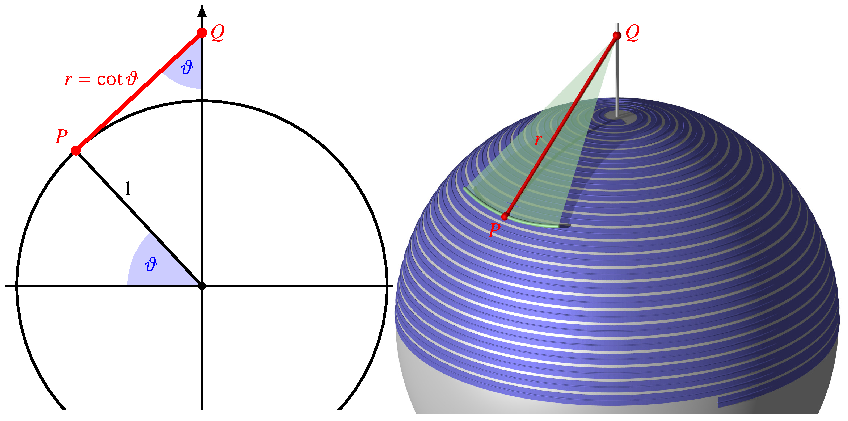
\includegraphics[width=\textwidth]{papers/fresnel/images/schale.pdf}
\caption{Schält man eine einen Streifen konstanter Breite beginnend am
Äquator von einer Kugel ab und breitet ihn in der Ebene aus, entsteht
eine Klothoide.
\label{fresnel:figure:schale}}
\end{figure}
\begin{figure}
\centering
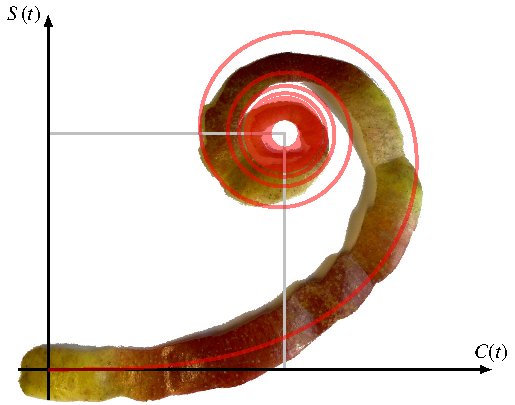
\includegraphics{papers/fresnel/images/apfel.pdf}
\caption{Klothoide erhalten durch Abschälen eines Streifens von einem
Apfel (vgl.~Abbildung~\ref{fresnel:figure:schale})
\label{fresnel:figure:apfel}}
\end{figure}
Schält man einen Streifen konstanter Breite beginnend parallel zum Äquator
von einer Kugel ab und breitet ihn in die Ebene aus, entsteht eine
Approximation einer Klothoide.
Abbildung~\ref{fresnel:figure:schale} zeigt blau den abgeschälten Streifen,
Abbildung~\ref{fresnel:figure:apfel} zeigt das Resultat dieses Versuches
an einem Apfel, das Youtube-Video \cite{fresnel:schale} des
Numberphile-Kanals illustriert das Problem anhand eines aufblasbaren
Globus.

Windet sich die Kurve in Abbildung~\ref{fresnel:figure:schale} $n$
mal um die vertikale Achse, bevor sie den Nordpol erreicht, dann kann
die Kurve mit der Funktion
\[
\gamma(t)
=
\begin{pmatrix}
\cos(t) \cos(t/n) \\
\sin(t) \cos(t/n) \\
\sin(t/n)
\end{pmatrix}
\]
parametrisiert werden.
Der Tangentialvektor
\[
\dot{\gamma}(t)
=
\begin{pmatrix}
-\sin(t)\cos(t/n) - \cos(t)\sin(t/n)/n \\
\cos(t)\cos(t/n) - \sin(t)\sin(t/n)/n \\
\cos(t/n)/n
\end{pmatrix}
\]
hat die Länge
\[
| \dot{\gamma}(t) |^2
=
\frac{1}{n^2}
+
\cos^2\frac{t}{n}.
\]
Die Ableitung der Bogenlänge ist daher
\[
\dot{s}(t)
=
\sqrt{
\frac{1}{n^2}
+
\cos^2\frac{t}{n}
}.
\]


Der Krümmungsradius des blauen Streifens, der die Kugel im Punkt $P$ bei 
geographischer $\vartheta$ berührt, hat die Länge der Tangente, die
die Kugel im Punkt $P$ berührt und im Punkt $Q$ durch die Achse der
Kugel geht (Abbildung~\ref{fresnel:figure:schale}).
Die Krümmung in Abhängigkeit von $\vartheta$ ist daher $\tan\vartheta$.




